\documentclass[11pt]{article}
\usepackage{charter}
\usepackage{graphicx}
\usepackage{hyperref}
\usepackage{mdframed}
\usepackage[margin=1in]{geometry}
\usepackage{amsmath,amssymb}

\hypersetup{
	colorlinks=true,
	linkcolor=blue,
	filecolor=magenta,
	urlcolor=cyan,
}

\begin{document}

%===================================================
% Title and Author Info
%===================================================
\begin{center}
{\Large\textsc{Compact Objects: White Dwarfs}} \\
\vspace{10pt}
{\large \textbf{Mentor:} Alex Urban} \\
{\small LIGO Laboratory, California Institute of Technology \\
Pasadena, CA 91125, USA \\
\href{mailto:aurban@ligo.caltech.edu}{\texttt{aurban@ligo.caltech.edu}}}
\end{center}

%%%%%%%%%%%%%%%%%%%%%%%%%%%%%%%%%%%%%%%%%%%%%%%%%%%

\section*{Electron Degeneracy Pressure and White Dwarfs}

\hspace{15pt} Last time, we started using a polytrope equation of state to model the interiors of white dwarf stars, which we can think of as a very dense gas of electrons bound to neutral atoms of carbon and oxygen. The electrons are dense enough that the Pauli exclusion principle exerts an \textit{electron degeneracy pressure} which overwhelms any thermal pressure in the star. What we found was that, using the equation of state and the condition for hydrostatic equilibrium, both the outer radius $R_*$ and the total mass $m_*$ of the star are completely determined by its central density, $\rho_c$.

\hspace{15pt} In real white dwarfs, the central density can exceed $\rho_c \sim$ 10$^6$ g/cm$^3$ (or about the mass of five wild elephants per teaspoonful of material). But, as we'll see in group, the average momentum per electron increases with density, meaning we have particles bouncing around at 1/3 the speed of light! For this reason, special relativity effects need to be accounted for.

\hspace{15pt} This problem set will introduce us to some of those relativistic effects and touch on a few crucial concepts in the astrophysics of white dwarfs. Most importantly, we will see that no white dwarf can have a mass bigger than about 1.4 $M_{\odot}$, which has surprisingly profound implications across astronomy. Beyond being an interesting digression, this will also build our intuition for the structure of very dense objects, and that's an intuition we're going to rely on next time when we start modeling neutron star interiors.

\vspace{5pt}

\begin{enumerate}

\item First, we'll take a step back and do a few neat ``back-of-the-envolope'' calculations. From the hydrostatic equilibrium equations for $dP/dr$ and $dm/dr$, argue that the central density, $\rho_{\rm c}$, and pressure, $P_{\rm c}$, inside a non-relativistic white dwarf are roughly on the order
\begin{equation}\label{eq:order_of_mag}
\rho_c \sim \frac{m_*}{R_*^3} \hspace{30pt} P_{\rm c} \sim \frac{Gm_*^2}{R_*^4}.
\end{equation}
In doing this, you can ignore any unitless factors of order 1. This kind of off-the-cuff argument is called a \textit{scaling law}, and these can be extraordinarily useful when we want to understand how a system behaves in the broadest sense.

\item Since ordinary main sequence stars are basically great big balls of gas whose behavior is dominated by thermal effects, we can model their internal equation of state as
\begin{equation}\label{eq:ideal}
P = K_0 T_{\rm c} \, \rho + \frac{4\sigma}{c} \, T_{\rm c}^4
\end{equation}
where $T_{\rm c}$ is the core temperature, $K_0 \sim$ 10$^4$ J/(kg K) is a constant that depends on the chemical makeup of the gas, and $\sigma$ is the Stefan-Boltzmann constant. The first term represents an ideal gas at temperature $T_{\rm c}$, while the second represents uniform radiation pressure. Using Eqs. \ref{eq:order_of_mag} and \ref{eq:ideal}, argue that any main sequence star's radius scales like
\begin{equation}\label{eq:m_R_stellar}
R_* \sim \frac{G m_*}{K_0 T_{\rm c}}.
\end{equation}
For stars the size of the Sun where $T_{\rm c} \sim$ 10$^7$ K, is radiation pressure important?

\item We'll want to see how $R_*$ compares with the star's Schwarzschild radius, $R_{\rm S} = 2Gm_*/c^2$. Express the ratio $R_*/R_{\rm S}$ in terms of $c$ and $T_{\rm c}$, and calculate this ratio explicitly for a few temperatures between 10$^6$ and 10$^9$ K. Do we have to worry about general relativity for main sequence stars?

\item Now, recall that our non-relativistic equation of state for white dwarfs had $P = K_1\rho^{\gamma}$, where $\gamma =$ 5/3 and
\begin{equation}\label{eq:K1}
K_1 = \frac{\hslash^2}{15\pi^2m_e} \left( \frac{3\pi^2}{n m_N} \right)^{5/3}
\end{equation}
is a constant, $m_e$ is the electron mass, $m_N$ the neutron mass, and $n$ the number of nucleons per electron. (In neutral atoms there is exactly one proton and one neutron for every electron, so we set $n=$ 2.) Using Eq. \ref{eq:order_of_mag} and the polytropic equation of state, argue that the outer radius of a white dwarf must roughly scale like
\begin{equation}\label{eq:m_R_nonrel}
R_* \sim \frac{K_1}{Gm_*^{1/3}}.
\end{equation}
This argument is valid for ``cold'' white dwarfs at $T=0$, which is a fine approximation since quantum effects dominate over thermal ones (see Fig. \ref{fig:EOS} if you need to be convinced.)

\item Notice that we're predicting the size of the white dwarf gets \emph{smaller} as the mass grows bigger. Can you qualitatively explain why this is?

\begin{figure}[!t]
\begin{mdframed}
\centering
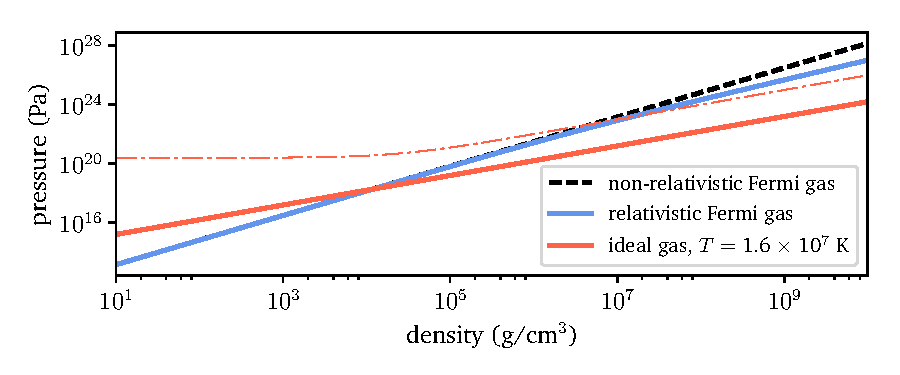
\includegraphics[scale=1]{white_dwarf/equation_of_state.pdf}
\caption{\label{fig:EOS} Model equations of state for a non-relativistic (black dashed curve) and fully relativistic (solid blue curve) gas of electrons at absolute zero, compared with the ideal gas equation of state at $T =$ 1.6 $\times$ 10$^7$ K (which represents the conditions at the core of the Sun). At white dwarf densities $\rho \sim$ 10$^4$-10$^8$ g/cm$^3$, we are justified in ignoring thermal effects because the electron degeneracy pressure clearly dominates. By \emph{several} orders of magnitude. (The light dashed-dotted curve represents the hottest and most massive stars, for which thermal pressure is comparable to electron degeneracy pressure.)}
\end{mdframed}
\end{figure}

\clearpage

\item So far, so good? Now let's have some fun! The full relativistic equation of state for a gas of electrons is fairly complicated, but fortunately there is a decent toy model approximation:
\begin{equation}\label{eq:EOS_rel}
P^{-2} = \left( K_1 \rho^{5/3} \right)^{-2} + \left( K_2 \rho^{4/3} \right)^{-2}
\end{equation}
where $K_1$ is the same as Eq. \ref{eq:K1} and
\begin{equation}\label{eq:K2}
K_2 = \frac{\hslash c}{12 \pi^2} \left( \frac{3\pi^2}{nm_N} \right)^{4/3}.
\end{equation}
This model effectively says that when you account for relativistic motion, the electrons have more and more states available to them as the density (and therefore, the total energy) increases. Eventually, there is a saturation point where the increase in pressure is shallower than one would expect without relativity, and we model all of this as a broken power law -- which is standard practice in astronomy.

\hspace{15pt} Using Eqs. \ref{eq:order_of_mag} and \ref{eq:EOS_rel}, argue that when we account for special relativity, the mass-radius scaling law becomes
\begin{equation}\label{eq:m_R_rel}
R_* \sim \frac{K_1}{Gm_*^{1/3}} \left( 1 - \frac{G^2m_*^{4/3}}{K_2^2} \right)^{1/2}.
\end{equation}
Compare this to Eq. \ref{eq:m_R_nonrel}. Where do you suppose this extra behavior comes from?

\item Compare the scaling laws in Eqs. \ref{eq:m_R_nonrel} and \ref{eq:m_R_rel} to the Schwarzschild radius, $R_{\rm S}$, by writing down the ratio $R_*/R_{\rm S}$ in each case. Do we have to worry about general relativity for white dwarfs?

\item Can you qualitatively explain what happens when $m_*$ approaches $M_{\rm Ch} \sim (K_2/G)^{3/2}$? We call this the \textit{Chandrasekhar mass limit}. Can you express the order of magnitude of $M_{\rm Ch}$ in terms of the fundamental constants $G$, $\hslash$, $m_N$, and $c$?

\item Write down order-of-magnitude estimates for the central density, $\rho_{\rm c}$, that you get using Eqs. \ref{eq:m_R_nonrel} and \ref{eq:m_R_rel}. Express these two different estimates in terms of $G$, $K_1$, $K_2$, and $m_*$, then compare both of them to the estimate you get from Eq. \ref{eq:m_R_stellar} at $T_{\rm c} \sim$ 10$^7$ K and $m_* \sim$ 1 $M_{\odot}$.

\item \textbf{Project Point:} Finally, let's stop dealing with orders of magnitude and fill in the specific details, using a simulation.

\hspace{15pt} Use Eq. \ref{eq:EOS_rel} and the Newtonian condition for hydrostatic equilibrium to numerically simulate $\rho(r)$ and $m(r)$ for a realistic white dwarf. By choosing a wide range of central densities, $\rho_c$, make a plot of $R_*$ as a function of $m_*$. Plot this for both the non-relativistic and the relativity-corrected cases, and compare this against those scaling laws we wrote down in the previous problems. In particular, fit your numerical results for $R_*(m_*)$ to the scaling laws we obtained and find the percent error of both models. Did our intuition guide us well? By how much were we off?

\hspace{15pt} In writing this simulation, note that your answer to problem (9) should tell you roughly what range of central densities to use, and how to space them out, in order to get a good sample of $R_*(m_*)$.

\end{enumerate}

%%%%%%%%%%%%%%%%%%%%%%%%%%%%%%%%%%%%%%%%%%%%%%%%%%%
\vspace{1000pt}

\section*{Things That Make You Go, ``Hmmm....''}

\begin{enumerate}

\item Note that only main sequence stars bigger than 10 $M_{\odot}$ which have spent all their hydrogen fuel can have core temperatures approaching $T_c\sim$10$^9$ K, beyond which nickel starts fusing into iron. But these atoms have the most binding energy per nucleon, so the fusion cannot produce any net energy, which renders the core inert and results in gravitational collapse. It's at this point that a supernova, powered by radioactive decay of nickel-56, marks the birth of a neutron star or black hole. But why can't this situation result in a white dwarf?

\item From Eq. \ref{eq:EOS_rel}, can you argue that special relativity should only make a difference at densities $\rho \gtrsim$ 10$^6$ g/cm$^3$?

\item The last equation of state (Eq. \ref{eq:EOS_rel}) is completely dominated by non-relativistic effects at very low densities ($\rho_{\rm c} \ll$ 10$^6$ g/cm$^3$) and by ultra-relativistic effects at very high densities ($\rho_{\rm c} \gg$ 10$^6$ g/cm$^3$). Can realistic white dwarfs \emph{ever} approach either of these limits?

\item I don't know about you, but I'm really geeking out over the fact that $M_{\rm Ch}$ combines Newtonian gravity (in the form of $G$), quantum mechanics ($\hslash$), and special relativity ($c$). It also just so happens to be a clean multiple of the Planck mass. There's \emph{totally} a reason for this that you'll hopefully see in a future course.

\item I'm also geeking out over the fact that Subrahmanyan Chandrasekhar derived this mass limit when he was 19 years old, and you've just accomplished the same feat!

\item We are almost fully equipped now to handle neutron stars -- in fact, much of what we've done here anticipates the astrophysics of neutron star interiors -- but we're still missing something. How will our model for neutron stars be different from white dwarfs? That is, in the most cartoonishly broad sense, what new physics will we need to account for to understand the structure of neutron stars? Remember the Schwarzschild radius, $R_{\rm S}$....

\end{enumerate}

\end{document}
